\documentclass[12pt]{article}
\usepackage{enumerate,mdframed}
\usepackage{notes}

\newcommand{\LHS}{\text{LHS}}
\newcommand{\RHS}{\text{RHS}}

\begin{document}
\title{Introduction to University Mathematics}
\maketitle

\section*{Sheet 1}
\subsection*{} % 1
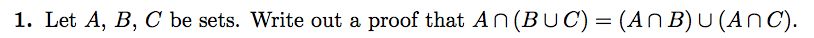
\includegraphics[width=400pt]{img/iulm-1-1.png}
\begin{mdframed}

Take the following things to have been defined already: intersection, union, subset.

Define $\LHS := A \cap (B \cup C)$ and $\RHS := (A \cap B) \cup (A \cap C)$.

We have to prove
\begin{enumerate}
\item that $\LHS \subset \RHS$, and
\item that $\RHS \subset \LHS$.
\end{enumerate}

\subsubsection*{Proof of (1)}
If $\LHS = \emptyset$, then (1) is true.

Alternatively, suppose $\LHS \neq \emptyset$ and let $x \in \LHS$. Then by the
definition of intersection, $x \in A$ and $x \in B \cup C$, and therefore by
the definition of union either $x \in B$ or $x \in C$.

Suppose $x \in B$. Then we have $x \in A$ and $x \in B$, so by the definition
of intersection $x \in A \cap B$. The RHS is the union of two sets, of which
$A \cap B$ is one. Therefore by the definition of union $x \in \RHS$.

Alternatively we can suppose $x \in C$. Since union and intersection commute,
$B$ and $C$ play equivalent roles and $x \in C$ leads to the same conclusion
that $x \in \RHS$ by an analogous argument to that above.

Therefore $\LHS \subset \RHS$.

\subsubsection*{Proof of (2)}
If $\RHS = \emptyset$, then (2) is true.

Alternatively, suppose $\RHS \neq \emptyset$ and let $x \in \RHS$. Then by the
definition of union, $x \in A \cap B$ or $x \in A \cap C$. Suppose
$x \in A \cap B$ (and label this ``supposition 1''). Then $x \in A$ and
$x \in B$. $x \in B \implies x \in B \cup Z$ for any set $Z$, so
$x \in B \cup C$, and therefore $x \in \LHS$.

Alternatively, at supposition 1, we could suppose $x \in A \cap C$. Due to
the symmetry resulting from commutativity of union and intersection, this also
leads to the conclusion $x \in \LHS$ by an identical argument.

Therefore $\RHS \subset \LHS$. \qed
\end{mdframed}


\subsection*{} % 2
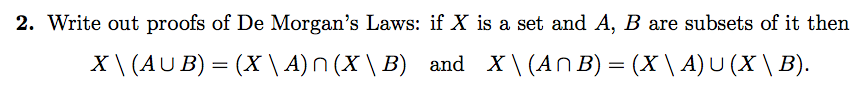
\includegraphics[width=400pt]{img/iulm-1-2.png}
\begin{mdframed}
\end{mdframed}

\newpage
\subsection*{} % 3
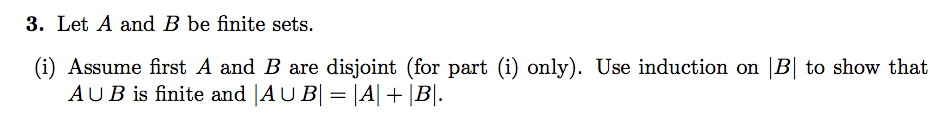
\includegraphics[width=400pt]{img/iulm-1-3.png}
\begin{mdframed}
First, observe that a set $X$ is finite if and only if $|X| \in \N$.

Second, observe that, if $|A \cup B| = |A| + |B|$ with $A$ and $B$ finite, then
$A \cup B$ is finite. Therefore it will suffice to show that
$|A \cup B| = |A| + |B|$.

We are told that $A$ and $B$ are finite.

Suppose $|B| = 0$. Then $B = \emptyset$ and $|A \cup B| = |A| = |A| + |B|$ as required.

Now suppose the desired result holds whenever $|B| = n$, i.e.
$|A \cup B| = |A| + n$. Specifically, let $B = X$ with $|X| = n$. We want to
show that when $|B|$ is increased to $n+1$, then $|A \cup B| = |A| + n+1$.

To increase $|B|$ to $n+1$, a new element $y \notin X$ must be added to
$B$. Also $y \notin A$ since we are told that $A$ and $B$ are disjoint. So now
\begin{align*}
  |A \cup B| &= |A \cup (X \cup \{y\})|\\
             &= |(A \cup X) \cup \{y\}| ~~~~\text{by associativity of union operation.}
\end{align*}
And since $y \notin X$ and $y \notin A$, $|(A \cup X) \cup \{y\}| = |A \cup X| + 1 = n + 1$.

Therefore by induction,
\begin{align*}
  |A \cup B| = |A| + |B|
\end{align*}
for finite and disjoint $A$, $B$. \qed
\end{mdframed}

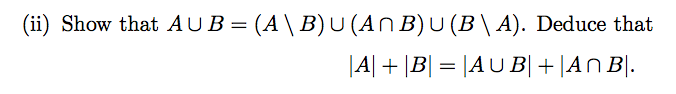
\includegraphics[width=300pt]{img/iulm-1-3-ii.png}
\begin{mdframed}

First, we show that
\begin{align}
  A \cup B ~~~ &\subset ~~~ (A \setminus B) \cup (A \cap B) \cup (B \setminus A).\label{3-forward}
\end{align}
Let $\LHS$ and $\RHS$ denote the expressions on the left- and right-hand sides
of the subset operator, respectively.

To show \eqref{3-forward}, first note that if $A \cup B = \emptyset$ then
\eqref{3-forward} is true. Alternatively suppose $A \cup B \neq \emptyset$ and
let $x \in A \cup B$. Note that since union and intersection commute, there are
symmetries in LHS and RHS, and in fact $A$ and $B$ are
exchangeable\footnote{need to define ``exchangeable''} in those
expressions. With that in mind, suppose that $x \in A$. Then either
$x \in A \cap B$ or $x \in A \setminus B$. So $x$ belongs to one of the three
sets in the union on the RHS. Alternatively we could have chosen $x \in B$, but
due to the symmetry described above we would be able to make an analogous
argument to conclude again that $x \in \RHS$. Thus we've shown that either LHS
is empty, or that any element of LHS is also an element of RHS, proving
\eqref{3-forward}.

Next we show that
\begin{align}
  (A \setminus B) \cup (A \cap B) \cup (B \setminus A) ~~~ &\subset ~~~ A \cup B. \label{3-backward}
\end{align}

Again, let $\LHS$ and $\RHS$ denote the expressions on the left- and right-hand
sides of the subset operator, respectively.

And again, if $\LHS = \emptyset$ then \eqref{3-backward} is
true. Alternatively, suppose $\LHS \neq \emptyset$. This implies that either
$A$ or $B$ is non-empty, since at least one of them has contributed at least
one element to the union. Suppose that $A \neq \emptyset$ and let $x \in
A$. Then $x \in A \cup B = \RHS$. Alternatively we could have chosen
$B \neq \emptyset$ and reached the same conclusion. Thus we've shown that
either LHS is empty, or that any element of LHS is also an element of RHS,
proving \eqref{3-backward}, and completing the proof of equality of LHS and
RHS.

Finally we are asked to deduce that $|A| + |B| = |A \cup B| + |A \cap B|$, or
equivalently $|A \cup B| &= |A| + |B| - |A \cap B|$. From the above, we know
that
\begin{align*}
  |A \cup B| &= |(A \setminus B) \cup (A \cap B) \cup (B \setminus A)|\\
             &= |(A \setminus B)| + |(A \cap B)| + |(B \setminus A)|,
\end{align*}
since the 3 sets are disjoint and union is associative. Now
$|X \setminus Y| = |X| - |X \cap Y|$\footnote{Does this need proof?}, therefore
\begin{align*}
  |A \cup B| &= |A| - |A \cap B| + |(A \cap B)| + |B| - |B \cap A|\\
             &= |A| + |B| - |A \cap B|.
\end{align*}
\qed
\end{mdframed}

\subsection*{} % 4
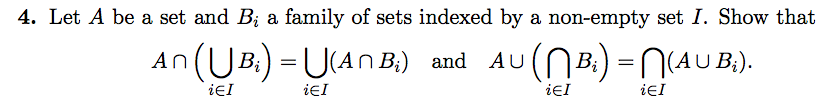
\includegraphics[width=400pt]{img/iulm-1-4.png}
\begin{mdframed}
\end{mdframed}

\subsection*{} % 5
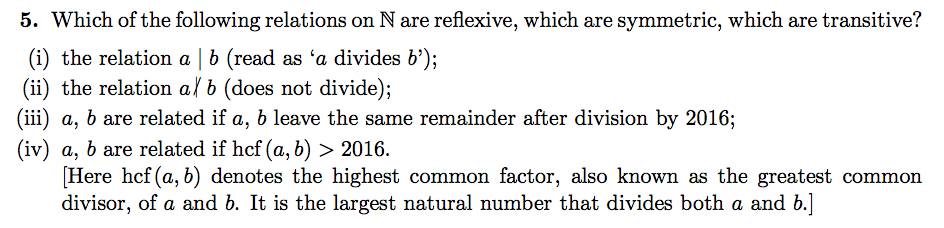
\includegraphics[width=400pt]{img/iulm-1-5.png}
\begin{mdframed}
\end{mdframed}

\subsection*{} % 6
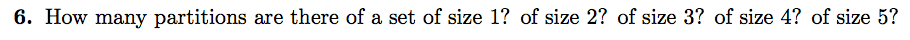
\includegraphics[width=400pt]{img/iulm-1-6.png}
\begin{mdframed}
\end{mdframed}

\subsection*{} % 7
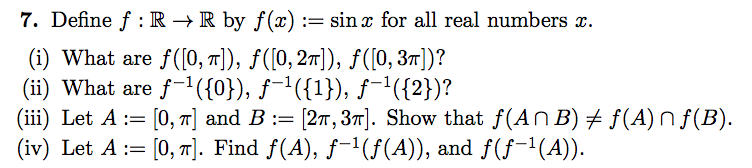
\includegraphics[width=400pt]{img/iulm-1-7.png}
\begin{mdframed}
\end{mdframed}

\subsection*{} % 8
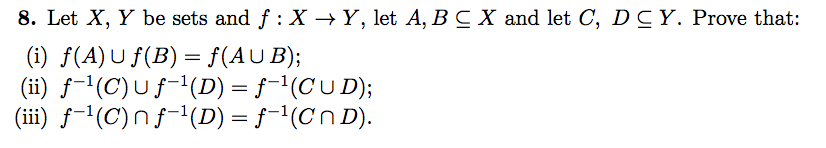
\includegraphics[width=400pt]{img/iulm-1-8.png}
\begin{mdframed}
\end{mdframed}

\subsection*{} % 9
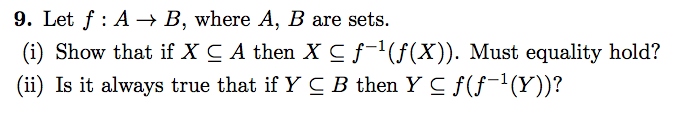
\includegraphics[width=400pt]{img/iulm-1-9.png}
\begin{mdframed}
\end{mdframed}

\subsection*{} % 10
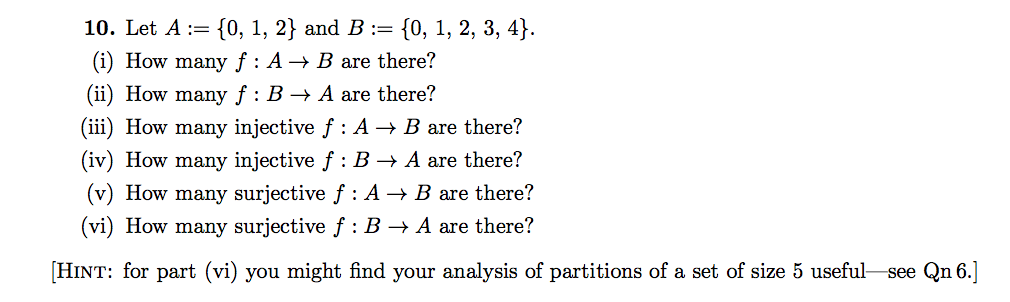
\includegraphics[width=400pt]{img/iulm-1-10.png}
\begin{mdframed}
\end{mdframed}

\newpage
\section{Sheet 2}
\subsection{}
\begin{mdframed}
  The attempted proof is flawed because it has the following form:
  \begin{enumerate}
  \item Suppose [the thing we are trying to prove]
  \item Deduce from this a tautology
  \item Conclude that [the thing we are trying to prove] is true.
  \end{enumerate}
  The problem is that it is possible to deduce a tautology from a false
  statement. For example $-1 = 1 \implies 1 = 1$ by squaring both sides.

  A correct proof follows.

  We are given that $a \geq 0, b \geq 0$. We start by noting that
  $0 \leq (a - b)^2$ is a tautology (true for all values of $a$ and
  $b$). Therefore
  \begin{align*}
              0 &\leq a^2 -2ab + b^2\\
    \implies  4ab &\leq a^2 + 2ab + b^2 = (a + b)^2\\
    \implies  2\sqrt{ab} &\leq a+b. \qed
  \end{align*}
\end{mdframed}

\subsection{}
\begin{mdframed}
  \begin{enumerate}[(a)]
  \item 2 is prime or 2 is odd.\\
    True. 2 is prime.
  \item 2 is prime or 2 is even.\\
    True. 2 is prime.
  \item If 2 is odd then 2 is prime.\\
    True. Premise is false so implication is true for all values of conclusion.
  \item If 2 is even then 2 is prime.\\
    True. Premise is true and conclusion is true, so implication is true.
  \item Forall $n \in \N$, if $n$ is a square number then $n$ is not prime.\\
    False, 1 is a square number yet not prime.
  \item Forall $n \in \N$, $n$ is not prime if and only if $n$ is a square number.\\
    False. 6 is not prime and yet not a square number.
  \item For all even primes $p > 2$, $p^2 = 2016$.\\
    True. There are no even primes greater than 2;
    $\forall ~ x \in \emptyset, ~p(x)$ is true for any predicate $p$.
  \end{enumerate}
\end{mdframed}


\subsection{}
\begin{mdframed}
Poorly-worded question. ``A card that has an even number on one side has a
vowel on the other'' might mean either of the following:
\begin{enumerate}
\item $\exists c: \text{even}(c) \text{~and~} \text{vowel}(c)$
\item $\text{even}(c) \implies \text{vowel}(c)$.
\end{enumerate}
If we assume the intended meaning is (2), then we could disprove the hypothesis
by finding an even card with a consonant. So we could try cards 2 and B. That
might lead to a counter-example. If it does not, then the experiment is
inconclusive, because a counter-example may exist in the unavailable cards in
the rest of the pack.

If we assume the intended meaning is (1), then we could try turning over 2 and
A. That might lead to an example confirming the truth of the hypothesis. If it
does not, then the experiment is inconclusive, because a confirmation may exist
in the unavailable cards in the rest of the pack.
\end{mdframed}
\subsection{}
\begin{mdframed}
\subsubsection*{Mathematical induction}
Consider a predicate function $p: \N \to \{\text{true},\text{false}\}$. We want to show
that $p(i)$ is true for all $i \in N$. In other words,

\textbf{Proposition}: $\forall ~ i \in N ~ p(i)$.\\

\textbf{Proof by induction}: First demonstrate that $p(0)$ is true. Next,
demonstrate that $p(i) \implies p(i+1)$.

\end{mdframed}

\subsection{}
\begin{mdframed}
  For all real numbers $a$ and positive reals $\epsilon$, there exists a
  positive real $\delta$ for which the following is true: for all real numbers
  $x$, $f(x)$ lies within a distance $\epsilon$ of $f(a)$ whenever $x$ lies
  within a distance $\delta$ of $a$.
\end{mdframed}

\subsection{}
\begin{mdframed}
  \begin{align*}
    \forall a \in \R: \forall x \in \R: \forall \epsilon \in \R^{>0}: \exists \delta \in \R^{>0}: |x - a| < \delta \implies |f(x) - f(a)| < \epsilon.
  \end{align*}
Yes it says much the same thing.
\end{mdframed}

\subsection{}

\newpage
\subsection{}
Let’s write $n = d_md_{m-1} \cdots d_2d_1d_0$ where $0 \leq d_i \leq 9$ for
$0 \leq i \leq m$ and $d_m \neq 0$, to mean that $n$ is an $(m+1)$-digit natural
number and the given string of digits is its decimal representation. Prove that
$n$ and $d_0 + d_1 + ··· + d_m−1 + d_m$ leave the same remainder
when divided by 9.\\
\begin{mdframed}
  We can sort of see this informally, in that every time we count through a
  block of 10 numbers, the remainder $\mod 9$ ``slips'' by 1. The coefficient
  in the 10s column records the ``number of slips''. When we get to 100, we've
  almost ``slipped through'' a whole block, and the 1 in the 100s column
  accounts for that.
  \subsubsection*{Proof}
  We have $n = \sum_{i=0}^m d_i 10^m$, and let $s(n) = \sum_{i=0}^m d_i$. Let
  $\bar{i}$ be the equivalence class of numbers that have $i \mod 9$ as their
  remainder when divided by 9 (clear way to make this definition?). The claim
  is that
  \begin{align*}
  \bar n = \bar{s(n)}.
  \end{align*}
  The key observation is that $\bar {10} = \bar 1$, so that the two summations
  expressions above end up mapping to the same equivalence class.

  To show this, note that the function that maps $i$ to $\bar i$ is a
  homomorphism, preserving both addition
  \begin{align*}
  \bar{i + j} = \bar i \oplus \bar j
  \end{align*}
  and multiplication
  \begin{align*}
  \bar{ij} = \bar i \otimes \bar j,
  \end{align*}
  where $\oplus$ and $\otimes$ denote the addition and multiplication
  operations on the set of equivalence classes. (The notation below doesn't
  always manage to distinguish between addition and multiplication on $\Z$
  versus the $\oplus$ and $\otimes$ operators.) Therefore
  \begin{align*}
    \bar n &= \bar{\sum_{i=0}^m d_i 10^m}
           = \sum_{i=0}^m \bar{d_i 10^m}
           = \sum_{i=0}^m \bar{d_i} \otimes \bar{10^m}
           = \sum_{i=0}^m \bar{d_i} \otimes \bar{10}~^m
           = \sum_{i=0}^m \bar{d_i} \otimes \bar{1}~^m\\
           &= \sum_{i=0}^m \bar{d_i} \otimes \bar{1}
           = \sum_{i=0}^m \bar{d_i}
           = \bar{\sum_{i=0}^m d_i} = \bar{s(n)}. \qed\\
  \end{align*}
  Alternatively,
  \begin{align*}
    n \mod 9 = s(n) \mod 9
    &\iff n - s(n) = 0 \mod 9\\
    &\iff \sum_{i=0}^m d_i 10^m - d_i = 0 \mod 9\\
    &\iff (10^m - 1)\sum_{i=0}^m d_i = 0 \mod 9\\
  \end{align*}
  which is true for all valid values of $m$ and $d_i$.
\end{mdframed}


\newpage
\subsection{}
Does there exist a positive integer $N$ which is a power of 2, and a different
positive integer $M$ obtained from $N$ by permuting its digits (in the usual
base 10 representation), such that $M$ is also a power of 2? Note that we do
not allow the base 10 representation of a positive integer to begin with 0.

\begin{mdframed}
  Not sure how to solve this, but here are a few observations:
  \begin{enumerate}
  \item If the two integers exist, they have the same number of digits in their
    decimal representation. I.e., they both lie in
    ${10^k,10^k + 2, \ldots, 10^{k+1} - 2}$ for some $k \geq 0$.
  \item For each ``order of magnitude'' $k$, there are either 3 or 4 powers of
    2.\footnote{To see this, note that we'll fit the most in if the first one
      is $10^k$ itself. (Powers of 2 are never actually a multiple of 10, but
      this will still give the upper bound.) Then
      $2\cdot 10^k, 2^2\cdot 10^k,2^3\cdot 10^k$ also fit in, giving
      4. Alternatively, the fewest that will fit in is when the first one is
      $2(10^k - 2)$. In this case we'll also get $2^2(10^k - 2)$ and
      $2^3(10^k - 2)$, giving 3.}
  \item We can re-phrase the question as follows:
    \begin{itemize}
    \item Visualize the powers of 2 belonging to the $k$-th order
      of magnitude as points in a $k$-dimensional grid with gridlines at
      $0, 1, 2, ...$. So for example, for $k=2$, the powers of 2 are
      $\{16, 32, 64\}$ and the points in the grid are
      $\{(1,6), (3,2), (6,4)\}$.
    \item Define an ``axis permutation'' of such a grid to be an operation that
      exchanges two of the coordinate axes, sending each occupied grid point to a
      new grid point.
    \item Define a ``congruent pair'' to be an ordered pair $(n_1, n_2)$ of
      powers of two, belonging to the same order of magnitude $k$, which has
      the following property: there exists some sequence of axis permutations
      after which the new location of $n_1$ is equal to the original location
      of $n_2$.
    \item Then we can rephrase the original question as: does there exist a $k$
      for which a congruent pair exists?
    \end{itemize}
  \end{enumerate}

  I looked up the proof:

  It's proof by contradiction. Suppose the pair of powers of 2 exist. The key
  observation is that we can use the mod 9 theorem: since the digits are the
  same (permuted) in the two integers, they sum to the same, and therefore the
  two integers are equal mod 9. Therefore their difference is a multiple of
  9. We know that the 4 values that are of the same length are $M, 2M, 4M,
  8M$. So if there's a pair that differ by permutation of their digits, then
  the difference between them must be $M, 3M$ or $7M$. In each case, that would
  mean that $M$ is a multiple of 9, and therefore not a power of 2. That
  contradiction proves it.

\end{mdframed}

\end{document}
